\chapter{GraphBLAS Operations}
\label{Sec:Operations}

The GraphBLAS operations are defined in the GraphBLAS math specification and summarized in 
Table~\ref{Tab:GraphBLASOps}.   In addition to methods that implement these
fundamental GraphBLAS operations, we support a number of variants that have been 
found to be especially useful in algorithm development.
A flowchart of the overall behavior of a GraphBLAS operation is shown 
in Figure~\ref{Fig:mxmFlowchart}.

\subparagraph{Associativity} 
We would like to emphasize that no GraphBLAS operation will imply a predefined order over any associative operators. Implementations of the GraphBLAS are encouraged to exploit associativity to optimize performance of any GraphBLAS operation. This holds even if the definition of the operation implies a fixed order for the associative operations.


\begin{table}[p]
\hrule
\begin{center}
\caption[A mathematical notation for the fundamental GraphBLAS operations 
supported in this specification.]{A mathematical notation for the fundamental GraphBLAS operations 
supported in this specification.  Input matrices $\matrix{A}$ and $\matrix{B}$ 
may be optionally transposed (not shown). Use of an optional accumulate with 
existing values in the output object is indicated with $\odot$.  Use of optional write 
masks and replace flags are indicated as $\matrix{C}\langle\matrix{M},r\rangle$ 
when applied to the output matrix, $\matrix{C}$.  The mask controls which values 
resulting from the operation on the right-hand side are written into the output 
object (complement and structure flags are not shown).  The ``replace'' 
option, indicated by specifying the $r$ flag, means that all values in the 
output object are removed prior to assignment. If ``replace'' is not specified, 
only the values/locations computed on the right-hand side and allowed by the 
mask will be written to the output (``merge'' mode).}
\label{Tab:GraphBLASOps}
~\\
\newcommand{\odotsp}{\hspace{-0.2cm}\odot\hspace{-0.18cm}}
\begin{tabular}{l|rcrcl}
{\sf Operation Name} & \multicolumn{5}{c}{Mathematical Notation}  \\
\hline
{\sf mxm}          & $\matrix{C}\langle\matrix{M},r\rangle$ & $=$ & $\matrix{C}$ & $\odotsp$ & $\matrix{A} \oplus.\otimes \matrix{B}$  \\
{\sf mxv}          & $\vector{w}\langle\vector{m},r\rangle$ & $=$ & $\vector{w}$ & $\odotsp$ & $\matrix{A} \oplus.\otimes \vector{u}$  \\
{\sf vxm}          & $\vector{w}^T\langle\vector{m}^T,r\rangle$ & $=$ & \hspace{-0.18cm}$\vector{w}^T$ & $\odotsp$ & $\vector{u}^T \oplus.\otimes \matrix{A}$  \\
{\sf eWiseMult}    & $\matrix{C}\langle\matrix{M},r\rangle$ & $=$ & $\matrix{C}$ & $\odotsp$ & $\matrix{A} \otimes \matrix{B}$  \\
                   & $\vector{w}\langle\matrix{m},r\rangle$ & $=$ & $\vector{w}$ & $\odotsp$ & $\vector{u} \otimes \vector{v}$  \\
{\sf eWiseAdd}     & $\matrix{C}\langle\matrix{M},r\rangle$ & $=$ & $\matrix{C}$ & $\odotsp$ & $\matrix{A} \oplus  \matrix{B}$  \\
                   & $\vector{w}\langle\matrix{m},r\rangle$ & $=$ & $\vector{w}$ & $\odotsp$ & $\vector{u} \oplus \vector{v}$  \\
{\sf extract}      & $\matrix{C}\langle\matrix{M},r\rangle$ & $=$ & $\matrix{C}$ & $\odotsp$ & $\matrix{A}(\grbarray{i},\grbarray{j})$ \\
                   & $\vector{w}\langle\matrix{m},r\rangle$ & $=$ & $\vector{w}$ & $\odotsp$ & $\vector{u}(\grbarray{i})$ \\
%{\sf extract} (column) & $\matrix{w}\langle\vector{m},r\rangle$ & $=$ & $\matrix{w}$ & $\odotsp$ & $\matrix{A}(\grbarray{i}, j)$ \\
{\sf assign}       & $\matrix{C}\langle\matrix{M},r\rangle(\grbarray{i},\grbarray{j})$ & $=$ & $\matrix{C}(\grbarray{i},\grbarray{j})$ & $\odotsp$ & $\matrix{A}$ \\
                   & $\vector{w}\langle\vector{m},r\rangle(\grbarray{i})$ & $=$ & $\vector{w}(\grbarray{i})$ & $\odotsp$ & $\matrix{u}$ \\
{\sf reduce} (row) & $\vector{w}\langle\vector{m},r\rangle$ & $=$ & $\vector{w}$ & $\odotsp$ & $\left[\oplus_j\matrix{A}(:,j)\right]$  \\
{\sf reduce} (scalar) & $s$ & $=$ & $s$ & $\odotsp$ & $\left[\oplus_{i,j}\matrix{A}(i,j) \right]$  \\
                      & $s$ & $=$ & $s$ & $\odotsp$ & $\left[\oplus_i\matrix{u}(i) \right]$  \\
{\sf apply}        & $\matrix{C}\langle\matrix{M},r\rangle$ & $=$ & $\matrix{C}$ & $\odotsp$ & $f_u(\matrix{A})$ \\
                   & $\vector{w}\langle\matrix{m},r\rangle$ & $=$ & $\vector{w}$ & $\odotsp$ & $f_u(\vector{u} )$  \\
\hline
{\sf apply(indexop)}     & $\matrix{C}\langle\matrix{M},r\rangle$ & $=$ & $\matrix{C}$ & $\odotsp$ & $f_{i}(\matrix{A},\mathbf{ind}(\matrix{A}),s)$ \\
                   & $\vector{w}\langle\matrix{m},r\rangle$ & $=$ & $\vector{w}$ & $\odotsp$ & $f_{i}(\vector{u},\mathbf{ind}(\vector{u}),s)$  \\
{\sf select  }     & $\matrix{C}\langle\matrix{M},r\rangle$ & $=$ & $\matrix{C}$ & $\odotsp$ & $\matrix{A}\langle f_{i}(\matrix{A},\mathbf{ind}(\matrix{A}),s)\rangle$ \\
                   & $\vector{w}\langle\matrix{m},r\rangle$ & $=$ & $\vector{w}$ & $\odotsp$ & $\vector{u}\langle f_{i}(\vector{u},\mathbf{ind}(\vector{u}),s)\rangle$  \\
\hline
{\sf transpose}    & $\matrix{C}\langle\matrix{M},r\rangle$ & $=$ & $\matrix{C}$ & $\odotsp$ & $\matrix{A}^T$ \\
{\sf kronecker}          & $\matrix{C}\langle\matrix{M},r\rangle$ & $=$ & $\matrix{C}$ & $\odotsp$ & $\matrix{A}  \kron \matrix{B}$  \\
%& & & \\
%& \multicolumn{3}{c}{Input/Output Operations} \\
%{\sf Matrix\_build}  & $\matrix{C}$ & $=$ & $\mathbb{S}^{m\times n}(\grbarray{i},\grbarray{j},\grbarray{v},\oplus_{dup})$ \\
%{\sf Vector\_build}  & $\vector{w}$ & $=$ & $\mathbb{S}^{n}(\grbarray{i},\grbarray{v},\oplus_{dup})$ \\
%{\sf Matrix\_extractTuples} & $(\grbarray{i},\grbarray{j},\grbarray{v})$ & $=$ & $\matrix{A}$ \\
%{\sf Vector\_extractTuples} & $(\grbarray{i},\grbarray{v})$ & $=$ & $\matrix{u}$ \\
\end{tabular}
\end{center}
\hrule
\end{table}

% Another take on the graphblas math notation

\setlength{\tabcolsep}{1.9pt}
%\renewcommand\arraystretch{0.85}

\begin{table}[htbp]
    \centering
    \begin{tabular}{llr@{}l}
        \hline
        \multicolumn{1}{c}{\bf op./method} & \multicolumn{1}{c}{\bf name}                          & \multicolumn{2}{c}{\bf notation} \\
        \hline
        \tt mxm                            & matrix-matrix multiplication                          & $\grbm{C} \grbmask{\grbm{M}}        $   & $\grbaccumeq{} \grbm{A} \grbplustimes \grbm{B}$  \\
        \tt vxm                            & vector-matrix multiplication                          & $\grbv{\grbv{w}} \grbmask{\grbv{m}} $   & $\grbaccumeq{} \grbv{u} \grbplustimes \grbm{A}$  \\
        \tt mxv                            & matrix-vector multiplication                          & $\grbv{w} \grbmask{\grbv{m}}        $   & $\grbaccumeq{} \grbm{A} \grbplustimes \grbv{u}$  \\
        \hline
        \multirow{2}{*}{\tt eWiseAdd}      & element-wise addition                                 & $\grbm{C} \grbmask{\grbm{M}} $          & $\grbaccumeq{} \grbm{A} \grbplus \grbm{B}$       \\
                                           & set union of patterns                                 & $\grbv{w} \grbmask{\grbv{m}} $          & $\grbaccumeq{} \grbv{u} \grbplus \grbv{v}$       \\
        \hline
        \multirow{2}{*}{\tt eWiseMult}     & element-wise multiplication                           & $\grbm{C} \grbmask{\grbm{M}} $          & $\grbaccumeq{} \grbm{A} \grbtimes \grbm{B}$      \\
                                           & set intersection of patterns                          & $\grbv{w} \grbmask{\grbv{m}} $          & $\grbaccumeq{} \grbv{u} \grbtimes \grbv{v}$      \\
        \hline
        \multirow{4}{*}{\tt extract}       & extract submatrix                                     & $\grbm{C} \grbmask{\grbm{M}} $          & $\grbaccumeq{} \grbm{A}(\grba{I}, \grba{J})$     \\
                                           & extract column vector                                 & $\grbv{w} \grbmask{\grbv{m}} $          & $\grbaccumeq{} \grbv{A}(:, \grbs{j})$            \\
                                           & extract row vector                                    & $\grbv{w} \grbmask{\grbv{m}} $          & $\grbaccumeq{} \grbv{A}(\grbs{i}, :)$            \\
                                           & extract subvector                                     & $\grbv{w} \grbmask{\grbv{m}} $          & $\grbaccumeq{} \grbv{u}(\grba{I})$               \\
        \hline
        \multirow{4}{*}{\tt assign}        & assign matrix to submatrix with mask for $\grbm{C}$   & $\grbm{C} \grbmask{\grbm{M}} (\grba{I},\grba{J}) $ & $\grbaccumeq{} \grbm{A}$              \\
                                           & assign scalar to submatrix with mask for $\grbm{C}$   & $\grbm{C} \grbmask{\grbm{M}} (\grba{I},\grba{J}) $ & $\grbaccumeq{} \grbs{s}$              \\
                                           & assign vector to subvector with mask for $\grbv{w}$   & $\grbv{w} \grbmask{\grbv{m}} (\grba{I}) $          & $\grbaccumeq{} \grbv{u}$              \\
                                           & assign scalar to subvector with mask for $\grbv{w}$   & $\grbv{w} \grbmask{\grbv{m}} (\grba{I}) $          & $\grbaccumeq{} \grbs{s}$              \\
        \hline
        \multirow{2}{*}{\tt apply}         & \multirow{2}{*}{apply unary operator}                 & $\grbm{C} \grbmask{\grbm{M}} $          & $\grbaccumeq{} \grbf{f}{\grbm{A}}$               \\
                                           &                                                       & $\grbv{w} \grbmask{\grbv{m}} $          & $\grbaccumeq{} \grbf{f}{\grbv{u}}$               \\
        \hline
        \multirow{4}{*}{\tt select}        & \multirow{4}{*}{apply select operator}                & $\grbm{C} \grbmask{\grbm{M}} $          & $\grbaccumeq{} \grbselect{\grbm{A}, \grbf{f}{\grbs{k}}}$            \\
                                           &                                                       & $\grbm{C} \grbmask{\grbm{M}} $          & $\grbaccumeq{} \grbselect{\grbs{low} \leq \grbm{A} \leq \grbs{up}}$ \\
                                           &                                                       & $\grbv{w} \grbmask{\grbv{m}} $          & $\grbaccumeq{} \grbselect{\grbv{u}, \grbf{f}{\grbs{k}}}$            \\
                                           &                                                       & $\grbv{w} \grbmask{\grbv{m}} $          & $\grbaccumeq{} \grbselect{\grbs{low} \leq \grbv{u} \leq \grbs{up}}$ \\
        \hline
        \multirow{3}{*}{\tt reduce}        & reduce matrix to column vector                        & $\grbv{w} \grbmask{\grbv{m}} $          & $\grbaccumeq{} \grbreduce{\grbplus}{\grbs{j}}{\grbm{A}}{\grbs{:},\grbs{j}}$ \\
                                           & reduce matrix to scalar                               & $\grbs{s} $                             & $\grbaccumeq{} \grbreduce{\grbplus}{\grbs{i}\grbs{j}}{\grbm{A}}{\grbs{i},\grbs{j}}$ \\
                                           & reduce vector to scalar                               & $\grbs{s} $                             & $\grbaccumeq{} \grbreduce{\grbplus}{\grbs{i}}{\grbm{u}}{\grbs{i}}$   \\
        \hline
        \multirow{1}{*}{\tt transpose}     & transpose                                             & $\grbm{C} \grbmask{\grbm{M}} $          & $\grbaccumeq{} \grbm{A}\grbt$                    \\
        \hline
        \tt kronecker                      & Kronecker multiplication                              & $\grbm{C} \grbmask{\grbm{M}}$           & $\grbaccumeq{} \grbkron{\grbm{A}, \grbm{B}}$     \\
        \hline\hline % operations above, methods below
        \multirow{2}{*}{\tt new}           & new matrix                                            & \multicolumn{2}{l}{$\grbnewmatrix{\grbm{A}}{\grbplaceholder{TYPE}}{\grbplaceholder{PRECISION}}{n}{m}$}  \\
                                           & new vector                                            & \multicolumn{2}{l}{$\grbnewvector{\grbv{u}}{\grbplaceholder{TYPE}}{\grbplaceholder{PRECISION}}{n}$}     \\
        \hline
        \multirow{2}{*}{\tt build}         & build matrix from index/value arrays                  & $\grbm{C}\ $                            & $\grbassign \left\{ \grba{I}, \grba{J}, \grba{X} \right\} $   \\
                                           & build vector from index/value arrays                  & $\grbv{w}\ $                            & $\grbassign \left\{ \grba{I}, \grba{X} \right\} $             \\
        \hline
        \multirow{2}{*}{\tt extractTuples} & \multirow{2}{*}{extract index/value arrays} & $ \left\{ \grba{I}, \grba{J}, \grba{X} \right\} $ & $\grbassign \grbm{A}$  \\
                                           &                                                       & $ \left\{ \grba{I}, \grba{X} \right\} $ & $\grbassign \grbv{u}$  \\
        \hline
        \multirow{2}{*}{\tt dup}           & duplicate matrix                                      & $\grbm{C} $                             & $\grbassign \grbm{A}$  \\
                                           & duplicate vector                                      & $\grbv{w} $                             & $\grbassign \grbv{u}$  \\
        \hline
        \multirow{2}{*}{\tt extractElement}& \multirow{2}{*}{extract scalar element}               & $\grbs{s} $                            & $\ = \grbm{A}(\grbs{i}, \grbs{j})$  \\
                                           &                                                       & $\grbs{s} $                             & $\ = \grbv{u}(\grbs{i})$   \\
        \hline
        \multirow{2}{*}{\tt setElement}    & \multirow{2}{*}{set element}                          & $\grbm{C}(\grbs{i}, \grbs{j}) $         & $\ = \grbs{s}$   \\
                                           &                                                       & $\grbv{w}(\grbs{i})$                    & $\ = \grbs{s}$   \\
        \hline
    \end{tabular}
    \caption{GraphBLAS operations and methods based on \cite{DBLP:journals/toms/Davis19}.
        \emph{Notation:}
        Matrices and vectors are typeset in bold, starting with uppercase ($\grbm{A}$) and lowercase ($\grbv{u}$) letters, respectively.
        Scalars including indices are lowercase italic ($\grbs{s}$, $\grbs{i}$, $\grbs{j}$) while arrays are uppercase italic ($\grba{X}$, $\grba{I}$, $\grba{J}$).
        $\grbplus$ and $\grbtimes$ are the addition and multiplication operators forming a semiring and default to conventional arithmetic $+$ and $\times$ operators.
        $\grbapply$ is the apply operator.
        Masks~$ \grbmask{\grbm{M}}$ and $\grbmask{\grbv{m}} $ are used to selectively write to the result matrix/vector. The complements of masks $\grbmask{\grbm{M}}$,
        $\grbmask{\grbv{m}}$
        can be selected with the negation symbol, denoted with
        $\grbmask{\grbneg \grbm{M}},$
        $\grbmask{\grbneg \grbv{m}}$,
        respectively.
        Masks
        with ``replace'' semantics (annihilating all elements outside the mask)
        are denoted with
        $\grbmaskreplace{\grbm{M}}$,
        $\grbmaskreplace{\grbneg \grbm{M}}$,
        $\grbmaskreplace{\grbv{m}}$, and
        $\grbmaskreplace{\grbneg \grbv{m}}$,
        The structure of the mask is denoted with
        $\grbmask{\grbstr{\grbm{M}}}$,
        $\grbmask{\grbneg \grbstr{\grbm{M}}}$,
        $\grbmask{\grbstr{\grbv{m}}}$, and
        $\grbmask{\grbneg \grbstr{\grbv{m}}}$.
    }
    \label{tab:graphblas-notation}
\end{table}




\begin{figure}[p]
    \hrule
    \begin{center}
        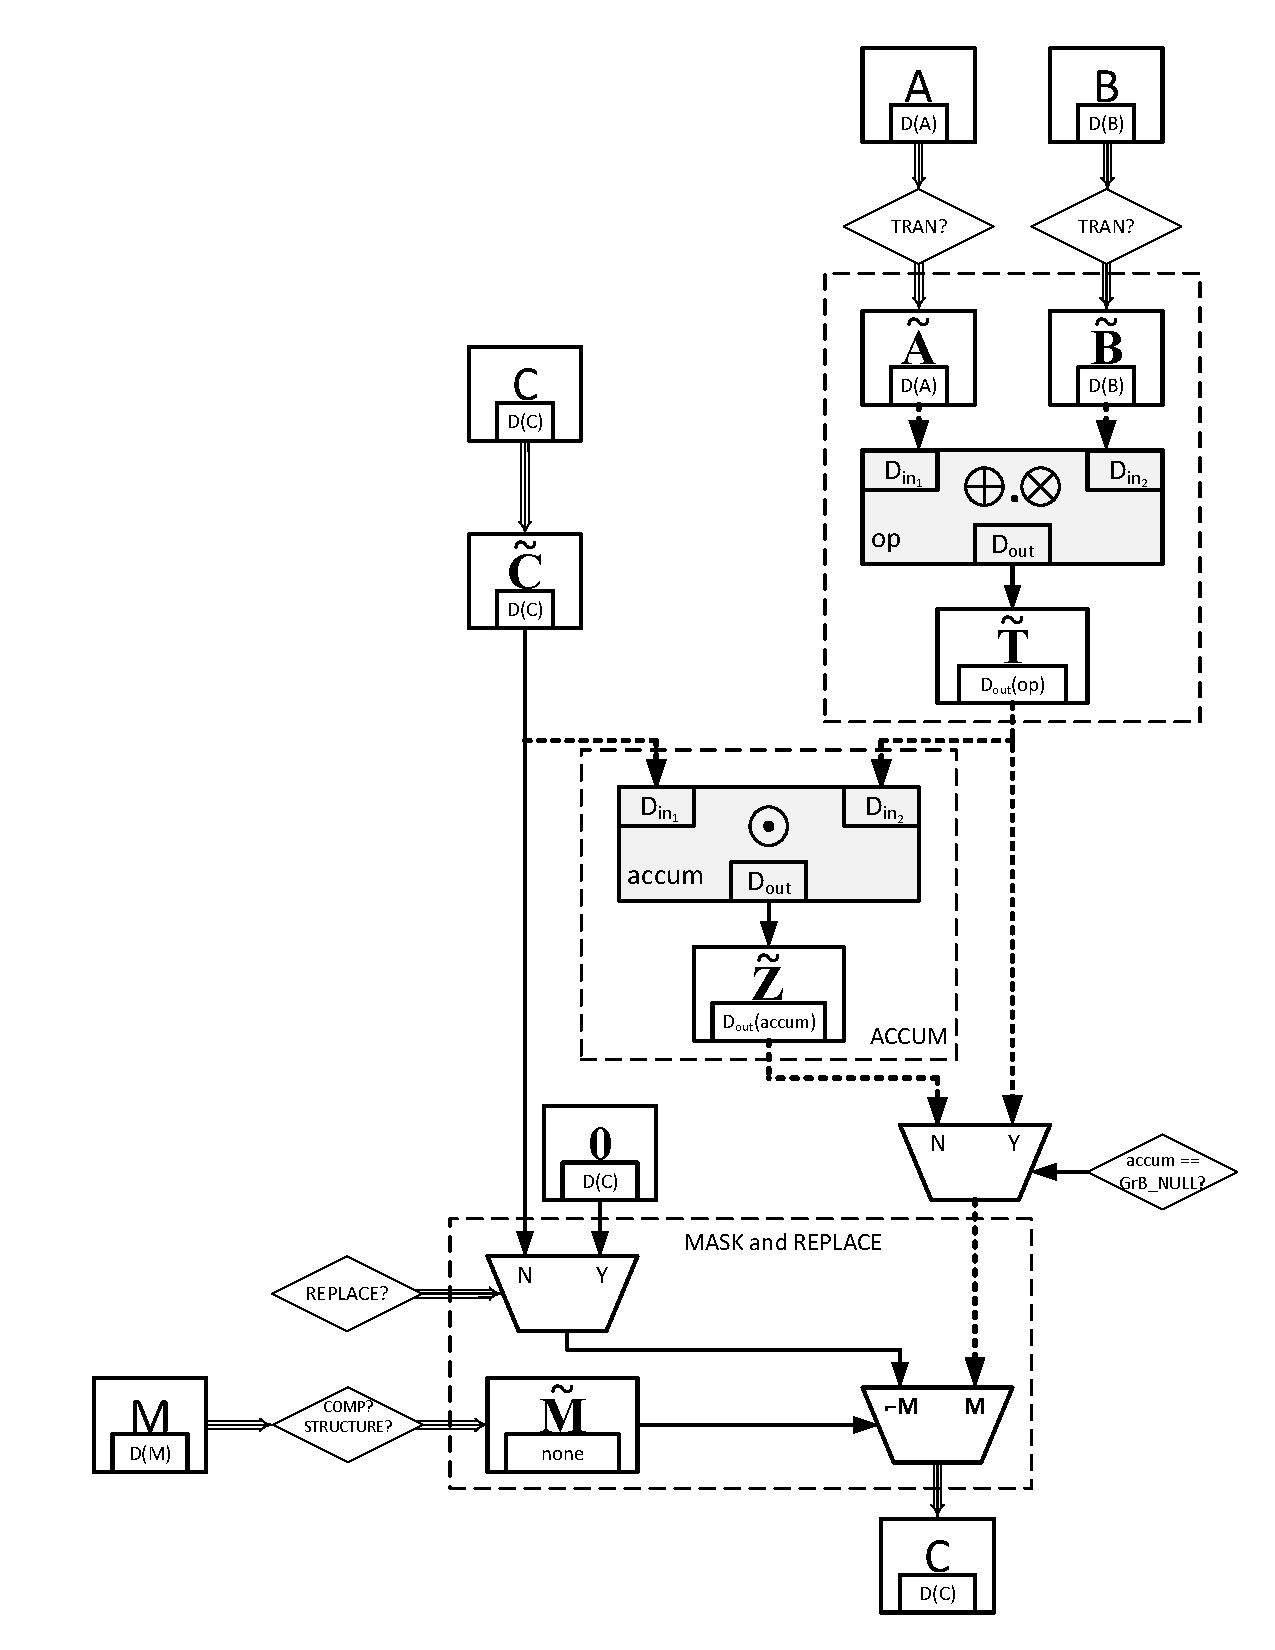
\includegraphics[width=5.5in]{mxm_operation_flowchart_1_3d.pdf}
    \end{center}
    \caption[Flowchart for the GraphBLAS operations.]{Flowchart for the GraphBLAS operations. Although shown specifically for
	the {\sf mxm} operation, many elements are common to all operations: such as the 
	``{\sf ACCUM}'' and ``{\sf MASK and REPLACE}'' blocks.  The triple arrows 
    ($\Rrightarrow$) denote where ``as if copy'' takes place (including both 
    collections and descriptor settings).  The bold, dotted arrows indicate
    where casting may occur between different domains.}
    \label{Fig:mxmFlowchart}
    \hrule
\end{figure}

\subparagraph{Domains \scott{and Casting?}:}
A GraphBLAS operation is only valid when the domains of the GraphBLAS objects are
mathematically consistent.  A programming language may define implicit casts 
between data types.  For example, {\sf float}s, {\sf double}s, and {\sf int}s can be 
freely mixed according to the rules defined for implicit casts in the C language.  It is the 
responsibility of the user to assure that these casts are appropriate for the language
in question.  For example, a cast to {\sf int} implies truncation of a floating 
point type.  Depending on the operation, this truncation error could lead to
erroneous results.  Furthermore, casting a wider type onto a narrower type can lead 
to overflow errors.  The specification of the GraphBLAS operations do not attempt to 
protect a user from these sorts of errors.

\subparagraph{Dimensions and Transposes:}
GraphBLAS operations also make assumptions about the numbers of dimensions and 
the sizes of vectors and matrices in an operation.   In this document we assume the
operands are \emph{shape compatible} for the mathematical definition of the operation 
being specified.  For example, when multiplying two matrices, 
$\matrix{C} = \matrix{A} \times \matrix{B}$, the number 
of rows of $\matrix{C}$ must equal the number of rows of $\matrix{A}$, the number of 
columns of $\matrix{A}$ must match the number of rows of $\matrix{B}$, and the number 
of columns of $\matrix{C}$ must match the number of columns of $\matrix{B}$.   
For most of the GraphBLAS operations involving matrices, optional transposition of
matrices can be specified. When matrices are optionally transposed \emph{shape compatibility}
is assumed to hold for the transposed matrix.

All GraphBLAS operations performed ``as if'' they are carried out in three sequential 
steps outlined as follows:

\begin{enumerate}[leftmargin=1.1in]
\item[\bf Base] The specific computation of a particular operation is carried out.  
An example is $\matrix{A}\oplus.\otimes\matrix{B}$ of {\sf mxm} or 
$\left[\oplus_{i,j}\matrix{A}(i,j) \right]$ of {\sf reduce}.  In this specification, 
the result of this step is stored in an intermediate matrix ($\tilde{\matrix{T}}$), 
vector ($\tilde{\vector{t}}$), or scalar ($\tilde{t}$).

\item[\bf Accumulation] All GraphBLAS operations support an optional accumulation step 
adding values in the existing output container (scalar, vector or matrix) with the 
results of the Base step.  In this specification, the result of this step is stored in 
an intermediate matrix ($\tilde{\matrix{Z}}$), vector ($\tilde{\vector{z}}$), or scalar ($\tilde{z}$).

\item[\bf Masking] For matrix and vector operations, the final result is written into 
the output container, possibly under control of a write mask -- either $\matrix{M}$ for 
matrices or $\vector{m}$ for vectors.  Scalar operations do not carry out this step.
\end{enumerate}

The Accumulation and Masking steps are common to most of the operations and are presented separately first.


%============================================================
%============================================================
\section{Optional Accumulation}

The mathematics...

\begin{itemize}
    \item[$\odot$] ({\sf IN}) An optional binary operator used for accumulating
    entries into existing $\matrix{C}$ entries, $\langle \bDout(\odot),\bDin1(\odot),\bDin2(\odot), \odot \rangle$.
\end{itemize}

\paragraph{Matrix accumulation}


The intermediate matrix $\matrix{\widetilde{Z}}$ is created as follows, using what is called a \emph{standard matrix accumulate}:
\begin{itemize}
    \item If ${\sf accum} = {\sf GrB\_NULL}$, then $\matrix{\widetilde{Z}} = \matrix{\widetilde{T}}$.

    \item If ${\sf accum}$ is a binary operator, then $\matrix{\widetilde{Z}}$ is defined as
        \[ \matrix{\widetilde{Z}} = \langle \bDout({\sf accum}), \bold{nrows}(\matrix{\widetilde{C}}), \bold{ncols}(\matrix{\widetilde{C}}),
        %\bold{L}(\matrix{\widetilde{Z}}) =
        \{(i,j,Z_{ij})  \forall (i,j) \in \bold{ind}(\matrix{\widetilde{C}}) \cup 
        \bold{ind}(\matrix{\widetilde{T}}) \} \rangle.\]

    The values of the elements of $\matrix{\widetilde{Z}}$ are computed based on the
    relationships between the sets of indices in $\matrix{\widetilde{C}}$ and 
    $\matrix{\widetilde{T}}$.
\[
    Z_{ij} = \matrix{\widetilde{C}}(i,j) \odot \matrix{\widetilde{T}}(i,j), \ \mbox{if}\  
    (i,j) \in  (\bold{ind}(\matrix{\widetilde{T}}) \cap \bold{ind}(\matrix{\widetilde{C}})),
\]
\[
    Z_{ij} = \matrix{\widetilde{C}}(i,j), \ \mbox{if}\  
    (i,j) \in (\bold{ind}(\matrix{\widetilde{C}}) - (\bold{ind}(\matrix{\widetilde{T}})
    \cap \bold{ind}(\matrix{\widetilde{C}}))),
\]
\[
    Z_{ij} = \matrix{\widetilde{T}}(i,j), \ \mbox{if}\  (i,j) \in  
    (\bold{ind}(\matrix{\widetilde{T}}) - (\bold{ind}(\matrix{\widetilde{T}})
    \cap \bold{ind}(\matrix{\widetilde{C}}))),
\]
where $\odot  = \bigodot({\sf accum})$, and the difference operator refers to set difference.
\end{itemize}



\paragraph{Vector accumulation}


The intermediate vector $\vector{\widetilde{z}}$ is created as follows, using what is called a \emph{standard vector accumulate}:
\begin{itemize}
    \item If ${\sf accum} = {\sf GrB\_NULL}$, then $\vector{\widetilde{z}} = \vector{\widetilde{t}}$.

    \item If ${\sf accum}$ is a binary operator, then $\vector{\widetilde{z}}$ is defined as
        \[ \vector{\widetilde{z}} = \langle \bDout({\sf accum}), \bold{size}(\vector{\widetilde{w}}),
        %\bold{L}(\vector{\widetilde{z}}) =
        \{(i,z_{i}) \ \forall \ i \in \bold{ind}(\vector{\widetilde{w}}) \cup 
        \bold{ind}(\vector{\widetilde{t}}) \} \rangle.\]

    The values of the elements of $\vector{\widetilde{z}}$ are computed based on the 
    relationships between the sets of indices in $\vector{\widetilde{w}}$ and 
    $\vector{\widetilde{t}}$.
\[
    z_{i} = \vector{\widetilde{w}}(i) \odot \vector{\widetilde{t}}(i), \ \mbox{if}\  
    i \in  (\bold{ind}(\vector{\widetilde{t}}) \cap \bold{ind}(\vector{\widetilde{w}})),
\]
\[
    z_{i} = \vector{\widetilde{w}}(i), \ \mbox{if}\  
    i \in (\bold{ind}(\vector{\widetilde{w}}) - (\bold{ind}(\vector{\widetilde{t}})
    \cap \bold{ind}(\vector{\widetilde{w}}))),
\]
\[
    z_{i} = \vector{\widetilde{t}}(i), \ \mbox{if}\  i \in  
    (\bold{ind}(\vector{\widetilde{t}}) - (\bold{ind}(\vector{\widetilde{t}})
    \cap \bold{ind}(\vector{\widetilde{w}}))),
\]
where $\odot  = \bigodot({\sf accum})$, and the difference operator refers to set difference.
\end{itemize}




%============================================================
%============================================================
\section{Optional Masking}

The mathematics...

\begin{itemize}
    \item[$\tilde{\matrix{M}}$] ({\sf IN}) $\in \mathbb{B}^{n\times m}$

	\item[{\sf Mask}] $\langle \bold{D}({\sf Mask}),\bold{nrows}({\sf Mask}),\bold{ncols}({\sf Mask}),\bold{L}({\sf Mask}) = \{(i,j,M_{ij}) \} \rangle$ (optional)
\end{itemize}

\paragraph{Masks: Structure-only, Complement, and Replace}

When a GraphBLAS operation supports the use of an optional mask, that mask is
specified through a GraphBLAS vector (for one-dimensional masks) or
a GraphBLAS matrix (for two-dimensional masks).  When a mask is used and the 
{\tt GrB\_STRUCTURE} descriptor value is not set, it is applied to the result 
from the operation wherever the stored values in the mask evaluate to true.  If
the {\tt GrB\_STRUCTURE} descriptor is set, the mask is applied to the result
from the operation wherever the mask as a stored value (regardless of that value).
Wherever the mask is applied, the result from the operation is either assigned 
to the provided output matrix/vector or, if a binary accumulation operation is 
provided, the result is accumulated into the corresponding elements of the provided 
output matrix/vector.

Given a GraphBLAS vector $\vector{v} = \langle D,N, \{ (i,v_i) \} \rangle$, a
one-dimensional mask is derived for use in the operation as follows:
\[
\vector{m} = 
\begin{cases}
\langle N, \{ \mathbf{ind}(\vector{v}) \} \rangle, & \mbox{if {\tt GrB\_STRUCTURE} is specified,} \\
\langle N, \{ i : \mbox{\tt (bool)}v_i = \true \} \rangle, & \mbox{otherwise}
\end{cases}
\]
where {\tt (bool)}$v_i$ denotes casting the value $v_i$ to a Boolean value (\true\ or \false).
Likewise, given a GraphBLAS matrix $\matrix{A} = \langle D, M, N, \{ (i,j,A_{ij}) \} \rangle$,
a two-dimensional mask is derived for use in the operation as follows:
\[
\matrix{M} = 
\begin{cases}
\langle M,N, \{ \mathbf{ind}(\matrix{A}) \} \rangle, & \mbox{if {\tt GrB\_STRUCTURE} is specified,} \\
\langle M,N, \{ (i,j) : \mbox{\tt (bool)}A_{ij} = \true \} \rangle, & \mbox{otherwise}
\end{cases}
\]
where {\tt (bool)}$A_{ij}$ denotes casting the value $A_{ij}$ to a Boolean value. 
(\true\ or \false)

In both the one- and two-dimensional cases, the mask may also have a subsequent 
complement operation applied ($Section$~\ref{Sec:Masks}) as specified in the 
descriptor, before a final mask is generated for use in the operation.

When the descriptor of an operation with a mask has specified that 
the {\sf GrB\_REPLACE} value is to be applied to the output ({\sf GrB\_OUTP}),
then anywhere the mask is not {\sf true}, the corresponding location in
the output is cleared.

$$
\matrix{C} \langle \matrix{M} \rangle \odot\!\!= \matrix{A} \oplus.\otimes \matrix{B}
$$

$$
\matrix{C} \langle \neg{\matrix{M}} \rangle \odot\!\!= \matrix{A} \oplus.\otimes \matrix{B}
$$

$$
\matrix{C} \langle s(\matrix{M}) \rangle \odot\!\!= \matrix{A} \oplus.\otimes \matrix{B}
$$

$$
\matrix{C} \langle s(\neg{\matrix{M}} \rangle \odot\!\!= \matrix{A} \oplus.\otimes \matrix{B}
$$


From the argument matrices, the internal mask used in 
the computation are formed ($\leftarrow$ denotes copy):
\begin{enumerate}
	\item Matrix $\matrix{\widetilde{C}} \leftarrow {\sf C}$.

	\item Two-dimensional mask, $\matrix{\widetilde{M}}$, is computed from
    argument {\sf Mask} as follows:
	\begin{enumerate}
		\item If ${\sf Mask} = {\sf GrB\_NULL}$, then $\matrix{\widetilde{M}} = 
        \langle \bold{nrows}({\sf C}), \bold{ncols}({\sf C}), \{(i,j), 
        \forall i,j : 0 \leq i <  \bold{nrows}({\sf C}), 0 \leq j < 
        \bold{ncols}({\sf C}) \} \rangle$.

		\item If {\sf Mask} $\ne$ {\sf GrB\_NULL},
        \begin{enumerate}
            \item If ${\sf desc[GrB\_MASK].GrB\_STRUCTURE}$ is set, then 
            $\matrix{\widetilde{M}} = \langle \bold{nrows}({\sf Mask}), 
            \bold{ncols}({\sf Mask}), \{(i,j) : (i,j) \in \bold{ind}({\sf Mask}) \} \rangle$,
            \item Otherwise, $\matrix{\widetilde{M}} = \langle \bold{nrows}({\sf Mask}), 
            \bold{ncols}({\sf Mask}), \\ \{(i,j) : (i,j) \in \bold{ind}({\sf Mask}) \wedge 
            ({\sf bool}){\sf Mask}(i,j) = \true\} \rangle$.
        \end{enumerate}

		\item	If ${\sf desc[GrB\_MASK].GrB\_COMP}$ is set, then 
        $\matrix{\widetilde{M}} \leftarrow \neg \matrix{\widetilde{M}}$.
	\end{enumerate}
\end{enumerate}

\paragraph{Matrix masking}


Finally, the set of output values that make up matrix $\matrix{\widetilde{Z}}$ 
are written into the final result matrix {\sf C}, using what is called
a \emph{standard matrix mask and replace}. 
This is carried out under control of the mask which acts as a ``write mask''.
\begin{itemize}
\item If {\sf desc[GrB\_OUTP].GrB\_REPLACE} is set, then any values in {\sf C} on
input to this operation are deleted and the content of the new output matrix,
{\sf C}, is defined as,
\[
\bold{L}({\sf C}) = \{(i,j,Z_{ij}) : (i,j) \in (\bold{ind}(\matrix{\widetilde{Z}}) 
\cap \bold{ind}(\matrix{\widetilde{M}})) \}. 
\]

\item If {\sf desc[GrB\_OUTP].GrB\_REPLACE} is not set, the elements of 
$\matrix{\widetilde{Z}}$ indicated by the mask are copied into the result 
matrix, {\sf C}, and elements of {\sf C} that fall outside the set 
indicated by the mask are unchanged:
\[
\bold{L}({\sf C}) = \{(i,j,C_{ij}) : (i,j) \in (\bold{ind}({\sf C}) 
\cap \bold{ind}(\neg \matrix{\widetilde{M}})) \} \cup \{(i,j,Z_{ij}) : (i,j) \in 
(\bold{ind}(\matrix{\widetilde{Z}}) \cap \bold{ind}(\matrix{\widetilde{M}})) \}.
\]
\end{itemize}

In {\sf GrB\_BLOCKING} mode, the method exits with return value 
{\sf GrB\_SUCCESS} and the new content of matrix {\sf C} is as defined above
and fully computed.
In {\sf GrB\_NONBLOCKING} mode, the method exits with return value 
{\sf GrB\_SUCCESS} and the new content of matrix {\sf C} is as defined above
but may not be fully computed. However, it can be used in the next GraphBLAS 
method call in a sequence.



\paragraph{Vector masking}


Finally, the set of output values that make up vector $\vector{\widetilde{z}}$ 
are written into the final result vector {\sf w}, using
what is called a \emph{standard vector mask and replace}. 
This is carried out under control of the mask which acts as a ``write mask''.
\begin{itemize}
\item If {\sf desc[GrB\_OUTP].GrB\_REPLACE} is set, then any values in {\sf w} 
on input to this operation are deleted and the content of the new output vector,
{\sf w}, is defined as,
\[ 
\bold{L}({\sf w}) = \{(i,z_{i}) : i \in (\bold{ind}(\vector{\widetilde{z}}) 
\cap \bold{ind}(\vector{\widetilde{m}})) \}. 
\]

\item If {\sf desc[GrB\_OUTP].GrB\_REPLACE} is not set, the elements of 
$\vector{\widetilde{z}}$ indicated by the mask are copied into the result 
vector, {\sf w}, and elements of {\sf w} that fall outside the set indicated by 
the mask are unchanged:
\[ 
\bold{L}({\sf w}) = \{(i,w_{i}) : i \in (\bold{ind}({\sf w}) 
\cap \bold{ind}(\neg \vector{\widetilde{m}})) \} \cup \{(i,z_{i}) : i \in 
(\bold{ind}(\vector{\widetilde{z}}) \cap \bold{ind}(\vector{\widetilde{m}})) \}. 
\]
\end{itemize}

In {\sf GrB\_BLOCKING} mode, the method exits with return value 
{\sf GrB\_SUCCESS} and the new content of vector {\sf w} is as defined above
and fully computed.  
In {\sf GrB\_NONBLOCKING} mode, the method exits with return value 
{\sf GrB\_SUCCESS} and the new content of vector {\sf w} is as defined above 
but may not be fully computed. However, it can be used in the next GraphBLAS 
method call in a sequence.

